% !TEX root = ../thesis.tex

\chapter{Využitie technologií v praxi}
\label{methodology}

Na vyriešenie problematiky nasadenia strojového učenia na platforme Kubernetes sú v tejto časti poskytnuté postupy na lokálne nasadenie na zariadeniach ako je laptop alebo stolný počítač. Jedna sa prevažne o platformu Kubeflow. Riešenia, ktoré sú poskytnuté sú mierne hardverovo záťažové, čo znamená, že sú vhodné pre zariadenia s lepším hardvérovým vybavením minimálne 8 GB veľkou operačnou pamäťou a s voľným priestorom na disku. Dodané postupy sú vhodné, či už pre slabšie zariadenia ale aj výkonovo silnejšie pre plné nasadenie platformy.

\section{Kubeflow}
Kubeflow ako platforma, je vhodná na nasadenie a vývoj strojového učenia. Primárne slúži pre inžinierov a vedcov, ktorý pracujú s dátami. Obsahuje viaceré komponenty, z ktorých si vývojári môžu vybrať, čo je pre ich používateľov najlepšie, čo znamená, že na nasadzovanie nie je potrebný každý jeden komponent.

\subsection{Komponenty}

Stavia na platforme Kubernetes ako systéme na nasadenie, škálovanie a správu zložitých systémov. Pomocou konfiguračných rozhraní Kubeflow, môžeme špecifikovať nástroje strojového učenia, potrebné pre náš pracovný postup. Potom môžeme nasadiť pracovný postup do rôznych cloudov, miestnych platforiem na experimentovanie a na produkčné použitie.\cite{web}

V tejto časti sú priblížené všetky šesť komponenty, ktoré tvoria Kubeflow.


\subsection*{Pipelines}

Pipelines sa používajú na vytváranie a nasadzovanie prenosných, škálovateľných, pracovných postupov strojového učenia založených na kontajneroch Docker. Pozostávajú z používateľského rozhrania na správu tréningových experimentov, úloh a chodov a z nástroja na plánovanie viackrokových pracovných postupov ML. Existujú aj dve súpravy SDK, jedna umožňuje definovať a manipulovať s kanálmi, zatiaľ čo druhá ponúka alternatívny spôsob interakcie Notebookov so systémom.\cite{pipe}

\subsection*{Notebooks}

Jupyter notebooks fungujú s Kubeflow veľmi dobre, pretože sa dajú ľahko integrovať s typickými mechanizmami overovania a kontroly prístupu. Používatelia môžu bezpečne a s istotou vytvárať notebookové moduly/servery priamo v klastri Kubeflow pomocou obrazov poskytnutých správcami a jednoducho odosielať úlohy s jedným uzlom v porovnaní s tým, že si musia všetko nakonfigurovať na svojom laptope.


\subsection*{Katib}

Katib je škálovateľný a rozšíriteľný framework na Kubernetes. Podporuje ladenie hyperparametrov a vyhľadávanie neurónovej architektúry. Umožňuje používateľom objaviť modely, ktoré sú rovnako dobré ako ručne vytvorené modely, bez toho, aby museli prejsť namáhavým manuánym procesom konfigurácie a opakovania. Katib organizuje optimalizáciu alebo vyhľadávanie neurónovej architektúry a presúva ju do sekcie s názvom Experiment. Algoritmy bežia interaktívnym spôsobom. Experiment definuje vyhľadávací priestor, cieľ metrík a maximálny počet iterácií. Katib hľadá iteratívne vo vyhľadávacom priestore, aby splnil cieľ metrík alebo aby dosiahol maximálny počet opakovaní. Katib podporuje dva rôzne mechanizmy – Hyperparameter Tuning a Neural Architecture Search. parafraze

Ladenie hyperparametrov je proces optimalizácie hodnôt hyperparametrov modelu s cieľom maximalizovať predikčnú kvalitu modelu. Príkladmi takýchto hyperparametrov sú rýchlosť učenia, hĺbka neurálnej architektúry (vrstvy) a šírka (uzly), epochy, veľkosť dávky, miera výpadkov a aktivačné funkcie. Toto sú parametre, ktoré sa nastavujú pred tréningom; na rozdiel od parametrov modelu (váhy a odchýlky) sa tieto nemenia počas procesu trénovania modelu.

\subsection*{Training operators}

Operátor Kubeflow pomáha nasadzovať, monitorovať a spravovať životný cyklus Kubeflow. Je zložený z Operator frameworku, čo je súprava nástrojov s otvoreným zdrojovým kódom na zostavovanie, testovanie, balenie operátorov a správu životného cyklu operátorov. Operátor Kubeflow používa KfDef ako svoj vlastný zdroj a kfctl ako základný nástroj na spustenie operátora.

Napríklad operátor k8s spadá pod Kubeflow. Tento operátor uľahčuje spúšťanie úloh tensorflow, či už sú distribuované alebo nedistribuované na kubernetes. TFjobs sú vlastným zdrojom kubernetes, ktorý sa používa na trénovanie alebo spustenie úloh trénovania na kubernetes. Kubeflow udržiava všetky tieto operátory a dá sa povedať, že kubeflow zhromažďuje také komponenty, ktoré uľahčujú spustenie kódu strojového učenia v rôznych formách v rámci Kubernetes. Takže potrebný je operátor pre TFJob, ktorý to bude monitorovať a sledovať. Nasadenie Kubeflow, dokáže rozšíriť nasadenia operátorov, a potom podľa toho definovať TFjobs a spustiť toľko, koľko tréningov je potrebné na klastri kubernetes.

\subsection*{Multi-Tenancy}

Po nainštalovaní a nakonfigurovaní Kubeflow sa predvolene pristupuje k primárnemu profilu. Profil vlastní menný priestor Kubernetes s rovnakým názvom spolu s kolekciou zdrojov Kubernetes. Používatelia majú prístup na zobrazenie a úpravu svojich primárnych profilov. Prístup k profilu je možné zdieľať s iným používateľom v systéme. Pri zdieľaní prístupu k profilu je na výber, aký prístup je možné poskytnúť na čítanie alebo prístup na čítanie/úpravu. Na všetky praktické účely pri práci s centrálnym ovládacím panelom Kubeflow je aktívny menný priestor priamo prepojený s aktívnym profilom.

\subsection*{Rozhranie}

Centrum riadenia komponentov, ktoré poskytuje používateľovi prístup k jednotlivým komponentom v klastri ako sú Pipelines, Notebooks, Katib, Artifact store a Multi-Tenancy.

Na nasledujúcom obrázku je možné vidieť rozhranie a niektoré komponenty, ktoré kubeflow ponúka.

\clearpage

\begin{figure}[h!]
    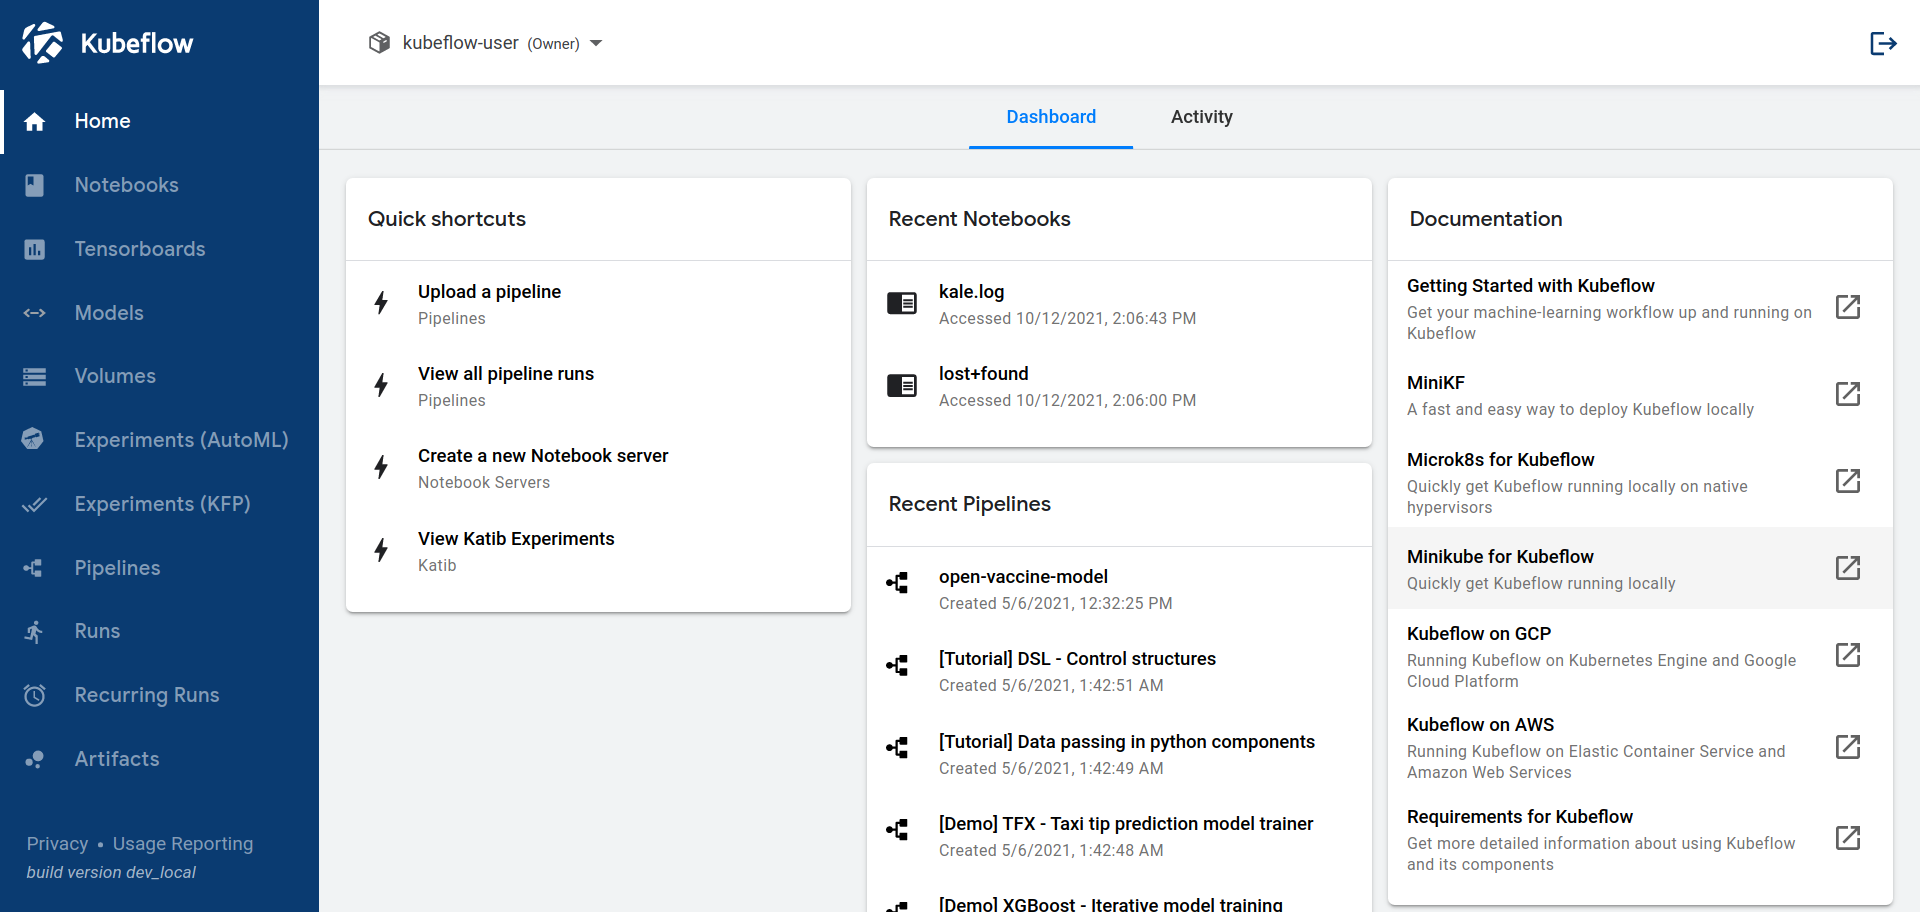
\includegraphics[width=\linewidth]{figures/Rozhranie}
    \caption{ Rozhranie Kubeflow }
\end{figure}

\subsection{Pracovný postup}

Postup pozostáva z viacerých krokov, taktiež z iterácie, ktorá je hlavným prvkom pri vyvíjaní sýtemu strojového učenia. Pri tomto postupe je potrebné vykonávať zmeny v parametroch aby sme dosiahli požadované výsledky. Následne si povieme niečo viac o týchto postupoch.

Ako prvé by sme mali vyvíjať model na základe predpokladov a testov. Môžeme ho opísať v nasledujúcich bodoch:\cite{web}

\begin{itemize}
    \item Identifikovanie problému, ktorý ma systém vyriešiť.
    \item Zbieranie dát, ktoré potrebujeme na trénovanie modelu.
    \item Vyberanie algoritmu a nakódovanie modelu.
    \item Experiment s údajmi a trénovanie modelu.
	\item Vyladenie parametrov.
\end{itemize}

Ďalej môžeme nasadiť systém, ktorý bude vykonávať tieto procesy:

\begin{itemize}
    \item Transformáciu údajov, ktoré náš systém potrebuje.
	\item Trénovanie modelu.
	\item Podanie modelu na online prevádzku.
	\item Monitorovanie výsledkov na úpravu a zmenu modelu.
\end{itemize}

\begin{figure}[!ht]
    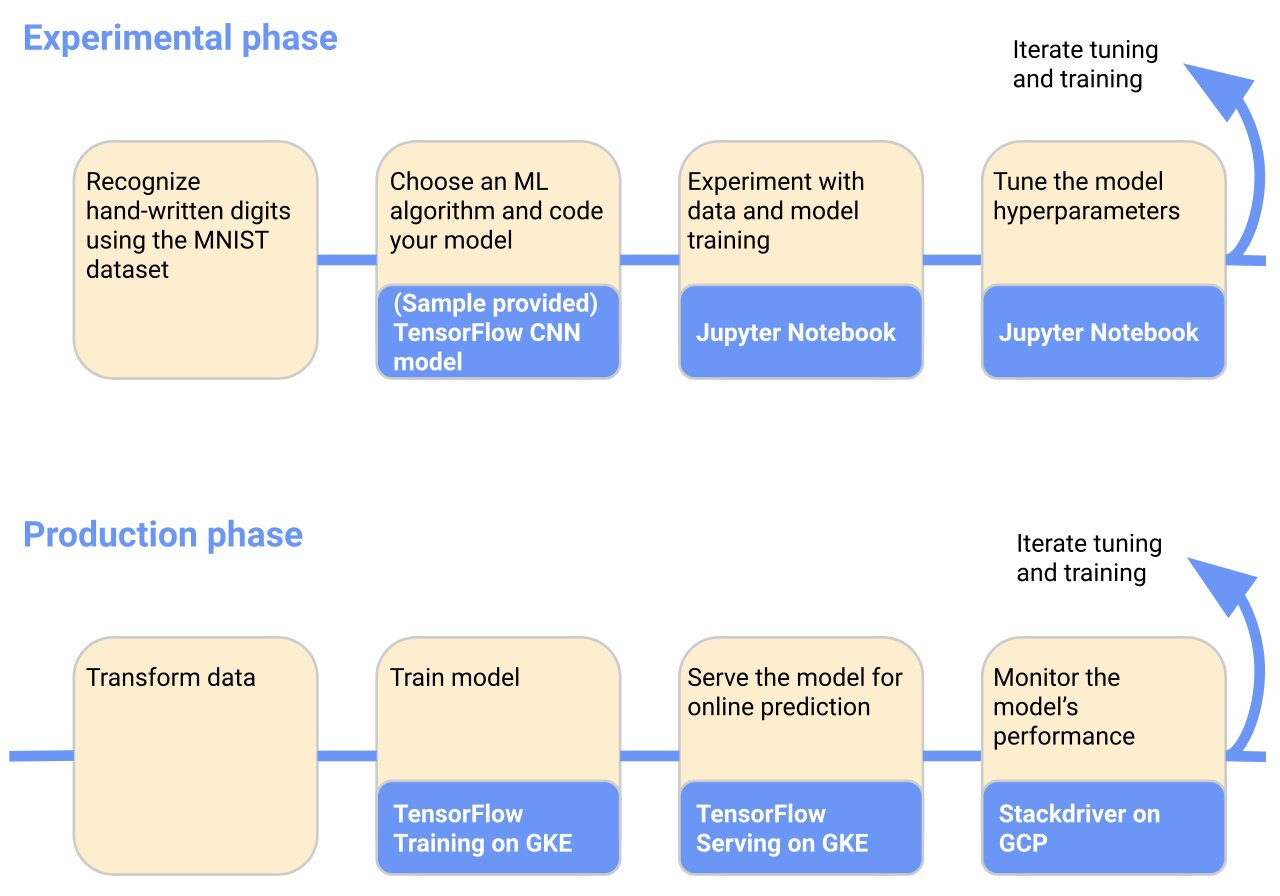
\includegraphics[width=.9\textwidth]{figures/kubeflowwork}
    \caption{\ Pracovné postupy \label{o:latex_friendly_zone}}
\end{figure}

\section{MiniKF}

Je softvér, vyvinutý spoločnosťou Arrikto, a to kombináciou viacerých služieb a nástrojov potrebných na spustenie úloh strojového učenia lokálne alebo vzdialene na platforme Kubernetes. Skladá sa z nástroja minikube na spustenie lokálnej platformy Kubernetes, samotného Kubeflow a platformy Rok, ktorá umožňuje spúšťanie stavových kontajnerov cez rýchle lokálne úložisko NVMe. MiniKF je lokálne nasadenie Kubeflow, ktoré je možné nainštalovať v priebehu minút. Po niekoľkých kliknutiach je možné začať experimentovať a dokonca spúšťať Machine Learning Pipelines.

Pred inštaláciou je potrebné nainštalovať VirtualBox a Vagrant. Je to softvér na vytváranie a udržovanie prenosných prostredí. Pre lokálne spustenie MiniKF je potrebné spĺňať minimálne požiadavky pre operačnú pamäť minimálne 12 GB, 2 jadra procesora a 50 GB voľného miesta na disku. Na operačnom systéme nezáleží, pretože je ho možné virtualizovať na rôznych operačných systémoch napríklad ako je Linux, macOS a Windows.

Inštalácia prebieha jednoducho a pozostáva z dvoch príkazov. Príkazom “vagrant init arrikto/minikf”  inicializujeme virtuálny počítač a príkazom “vagrant up” sa zapne virtuálny počítač. Kubeflow je poháňaný prostredníctvom Kubernetes na tomto virtuálnom počítací. Ak je virtuálny počítač pripravený spusti sa na ňom skript a následne je možné sa pripojiť cez internetový prehliadač k danému počítaču, kde sa spustí nastroj, ktorý developuje serie softvérových balíčkov potrebné na spustenie Kubeflow. Po reštartovaní počítača sa dáta nestratia, stačí zopakovať postup a je možné sa vrátiť k začatej práci.

\section{Charmed}

Pri developovaní Kubeflow sa pri tomto spôsobe využíva Juju Charm. Juju Charm je bezplatný aplikačný nástroj na modelovanie aplikácii s otvoreným zdrojovým kódom vyvinutý spoločnosťou Canonical, je známy aj ako štruktúrovaný balík konfiguračných súborov YAML a skriptov pre softvérový komponent, ktorý umožňuje Juju nasadiť a spravovať softvérový komponent ako službu podľa osvedčených postupov. Poskytuje centrálny pohľad na operátorov Kubernetes v nasadení, konfigurácií, rozsahu a stavu každého z nich a integračných liniek medzi nimi. Sleduje potenciálne aktualizácie a inovácie pre každého operátora a koordinuje tok udalostí a správ medzi operátormi.

Tento spôsob je vhodný najmä pre používateľov s operačným systémom Ubuntu. Samozrejme ho je možné použiť aj na iných operačných systémoch použitím virtualizácie, odporúča sa využiť Multipass, nenáročného správcu virtuálnych počítačov Ubuntu. Poskytuje virtualizáciu využitím Hyper-V alebo VirtualBoxu. Minimálne požiadavky závisia od verzie Kubeflow a to pri verzii full sú väčšie, minimálne 16 GB operačnej pamäte a 60 GB voľného miesta na disku. Full verzia poskytuje všetky služby napríklad Katib a Jupyter Notebooks. Verzia s označením lite bola vytvorená pre používateľov, ktorí pracujú v prostredí s obmedzenými zdrojmi a mal by fungovať dobre pri 8 GB operačnej pamäte a 50 GB dostupných na disku. Zachováva užívateľsky dashboard, ktorý je vhodný najmä pre začiatočníkov s lepšou interakciou. Tento balík je orientovaný najmä na nasadenie na systémoch ako notebook. Poslednou a najľahšou verziou je edge, ktorá neobsahuje dashboard a je vhodná pre tých, ktorí vyžadujú vlastných operátorov alebo pre zariadenia so slabšími výkonom. Na spustenie postačuje 4 GB operačnej pamäte. Pri každej verzii sú potrebné 4 jadra procesora. Je možné tieto verzie aj editovať, ak neobsahujú niečo potrebné a to upravením YAML súboru.

Prvým krokom je nainštalovať Multipass, ak postup sa vykonáva na zariadení, ktorý ma operačný systém iný ako Ubuntu. Pre správne fungovanie sa využíva MicroK8s pre spravovanie klastra s 1.21 verziou Kubernetes. Je dostupná aj novšia verzia s označením 1.22, ktorá zatiaľ nepodporuje Kubeflow. Aby ďalšie príkazy fungovali bez použitia sudo je treba pridať používateľa do skupiny. Ak je Kubernetes pripravený, dostupné sú viaceré služby. Aby sa navzájom našli aplikácie, úložisko, prístup ku komponentom Kubeflow a aplikácii na vyrovnávanie záťaže MetalLB je nutné pridať DNS službu. Pred ďalšími krokmi sa kontroluje, či boli služby povolené. Pre developovanie Kubeflow platformy je nevyhnutný Juju nastroj. Jeho inštalácia je pomerne jednoduchá, pretože sa inštaluje z balíka využitím systému snap na spravovanie balíčkov. Spustenie príkazu na nasadenie ovládača Juju do Kubernetes pre ovládanie komponentov Kubeflow a odporúča sa taktiež nastaviť špecificky model. Po Juju nasleduje proces nasadenia Kubeflow a je treba vyčkať pokiaľ sa jednotlivé aplikácie a komponenty pripravia a budú môcť medzi sebou komunikovať. Pre prístup k dashboardu nakonfigurovanie niektorých komponentov je nevyhnutné s povolenou adresou URL. K dispozícii je aj možnosť nastavenia mena a hesla. Na záver je možné zobraziť dashboard v prehliadači s URL, ktorú sme nakonfigurovali. Ak sa využíva Multipass pre získanie prístupu je vhodné vytvoriť pripojenie použitím SSH so zapnutým SOCKS proxy.

\section{Pipelines}

Tento spôsob je vhodný, vtedy ak je žiadaná práca výhradne s Kubeflow pipelines. Cieľom je nasadiť pipelines na lokálnom klastri. Na nasadenie nie sú nutné žiadne virtualizačné programy a postup je v celku jednoduchý, pretože sú tým výnimočne. Kubeflow pipelines sú známe kontajnerizáciou, čo znamená, že bude sa používať Docker na vytváranie kontajnerov. Požiadavky na spustenie nie sú náročne, pre operačnú pamäť si vyžadujú minimálne 8 GB a 2 jadra procesora. Nástroj kind je kľúčový, slúži na vytvorenie lokálneho Kubernetes klastra využitím Dockera. Taktiež by bolo dobre poznamenať, že Docker vyžaduje Windows Subsystem for Linux (WSL), ktorý slúži pre natívny beh linuxových spustiteľných súborov v prostredí Windows. Pre správny postup inštalácie sa požaduje aj kubectl, ktorý sa používa na komunikáciu s klastrom vyžitím príkazového riadka a Git.

Na začiatok je potrebné nainštalovať nástroj kind. Inštalácia na operačnom systéme Windows je veľmi jednoduchá a pozastaví z niekoľko príkazov, pripadne je možné použiť Chocolatey, ktorý je vhodný na inštaláciu balíčkov na systéme Windows. Ďalším krokom je vytvorenie klastra príkazom “kind create cluster”.  Kind spusti klaster Kubernetes pomocou vopred vytvoreného obrazu. Samozrejmosťou je použitie vlastného obrazu. Nasadenie pipelines sa vykoná spustením príkazov, ktoré stiahnu všetko potrebne z gitu a treba počkať niekoľko minút pokiaľ prebehne nasadenie všetkých komponentov potrebných pre pipelines a následne posledným krokom je presmerovanie portov. Po presmerovaní je Kubeflow dostupný otvorením internetového prehliadača na adrese „http://localhost:8080/“.


\clearpage